
\chapter{Mutations affecting the mean open time}
\label{mot_chapter}

In the simplest case of Markov models of the form
\begin{equation}
C\underset{k_{co}}{\overset{k_{oc}}{\leftrightarrows}}O, \label{mot_markov}
\end{equation}
we have studied mutations leading to an increased open probability by increasing
the rate from closed (C) to open (O), given by $k_{co}$. We refer to these as 
CO-mutations and for such mutations we
have successfully derived closed state blockers represented as
\begin{equation}
B\underset{k_{bc}}{\overset{k_{cb}}{\leftrightarrows}}C\underset{\mu
k_{co}}{\overset{k_{oc}}{\leftrightarrows}}O, \label{mot_cl}
\end{equation}
where $\mu\geqslant1$ is the mutation severity index and $\mu=1$
represents the wild type. These blockers can completely repair the equilibrium
open probability of the mutant by adjusting the ``on rate'' divided by the
``off rate'' of the drug given by
\[
\delta_{c}=\frac{k_{cb}}{k_{bc}}
\]
(see, e.g., page \pageref{d_c}). The remaining degree of freedom can be found
using probability density systems and the resulting drugs have been proven to
work exceptionally well in theoretical computations.

There is, however, another way of modeling increased equilibrium open
probability. Rather than increasing the rate from C to O, we can reduce the
rate from O to C:
\begin{equation}
C\underset{k_{co}}{\overset{k_{oc}/\mu}{\leftrightarrows}}O,
\end{equation}
where again $\mu\geqslant1$ is referred to as the mutation severity index. 
This type of mutation is referred to as an OC-mutation and the
equilibrium open probability for this Markov model is given by
\[
o=\frac{1}{1+\frac{k_{oc}/\mu}{k_{co}}},
\]
which clearly increases for increasing values of $\mu.$ Formally, we can carry out
the same math to devise a closed state drug that completely repairs the
equilibrium open probability of the mutant; however, when this drug is put into the
probability density system to determine the remaining degree of
freedom of the drug, we quickly observe that the task is impossible and the
theoretical drug does not provide significant improvement.

The core difficulty here is that a CO-mutation does not
change the mean open time of the channel. A closed state blocker is therefore
well suited because such a blocker does not affect the mean open time. 
However, for an OC-mutation,
an increased mean open time is part of the problem and a closed state blocker
is not the solution, simply because it cannot affect the mean open time. Rather, an open state blocker must be used.

In this chapter, we will explain the notion of mean open time and study
mutations that lead to an increased open probability \textit{and} an increased mean
open time. We will show that open state blockers are optimal for such mutations.

\section{The mean open time}

Let us briefly recall the interpretation of the Markov model
\[
C\underset{k_{co}}{\overset{k_{oc}}{\leftrightarrows}}O.
\]
This scheme means that if the channel is closed (C), the probability of
changing the state from closed to open (O) in a small time interval $\Delta t$ is
given by $k_{co}\Delta t.$ Clearly, this interpretation only holds for short
time intervals, since the probability cannot exceed one. Note also that if the
rate $k_{co}$ increases, this leads to an increased probability of moving from C
to O during the time step $\Delta t.$ Similarly, $k_{oc}\Delta t$ denotes the
probability of moving from the open state to the closed state in the time step
$\Delta t.$

Suppose that the channel is open at time $t=0.$ The probability that the
channel remains open after a short time step $\Delta t$ is given by
\[
p_{1}=1-k_{oc}\Delta t.
\]
If we take another time step, the probability that the channel is still open
at time $t=2\Delta t$ is given by
\[
p_{2}=p_{1}\left(  1-k_{oc}\Delta t\right)  =\left(  1-k_{oc}\Delta t\right)
^{2}
\]
and so on. At time $t=n\Delta t,$ the probability of the channel still being
open is given by
\[
p_{n}=\left(  1-k_{oc}\Delta t\right)  ^{n}.
\]
If we now introduce time given by
\[
t=n\Delta t,
\]
we have
\[
\left(  1-k_{oc}\Delta t\right)  ^{n}=\left(  1-k_{oc}\Delta t\right)
^{\frac{t}{\Delta t}}.
\]
The probability of closing a channel that is in the open state during a
time step is given by $\Delta tk_{oc}$ and therefore the probability of
closing a channel that has remained open for $n$ time steps is given by
\[
\Delta tk_{oc}\left(  1-k_{oc}\Delta t\right)  ^{\frac{t}{\Delta t}}.
\]
The expected open time is therefore given by
\[
\sum_{n=1}^{\infty}n\Delta t\left(  1-k_{oc}\Delta t\right)  ^{\frac{t}{\Delta
t}}\Delta tk_{oc}.
\]
If we go to the limit of $\Delta t\rightarrow0$ in this expression, we find
that
\[
\sum_{n=1}^{\infty}n\Delta t\left(  1-k_{oc}\Delta t\right)  ^{\frac{t}{\Delta
t}}\Delta tk_{oc}\overset{\Delta t\rightarrow0}{\longrightarrow}\int
_{0}^{\infty}tk_{oc}e^{-k_{oc}t}dt=\frac{1}{k_{oc}}
\]
and therefore we have found that the mean open time is given by
\begin{equation}
\tau_{o}=\frac{1}{k_{oc}}. \label{tau_o}
\end{equation}


\subsection{Mean open time for more than one open state}
\label{mot_many}


We have seen that the mean open time for a Markov model of the form
\[
C\underset{k_{co}}{\overset{k_{oc}}{\leftrightarrows}}O
\]
is given by
\begin{equation}
\tau_{o}=\frac{1}{k_{oc}}. 
\end{equation}
It is straightforward to extend the argument above to see that, for a Markov
model of the form 
\[
C\underset{k_{co}}{\overset{k_{oc}}{\leftrightarrows}}O\underset{k_{ob}}{\overset{k_{bo}}{\leftrightarrows}}B,
\]
the mean open time is given by
\begin{equation}
\tau_{o}=\frac{1}{k_{oc}+k_{ob}}. 
\end{equation}
But what happens if there is more than one open state? This situation
will become relevant below, where we consider models including a burst mode.
The models contain at least two open states. To understand the mean
open time in the presence of more than one open state, we consider the
generic extension illustrated in Figure \ref{o2}.


\begin{figure}[ptb]
\begin{center}
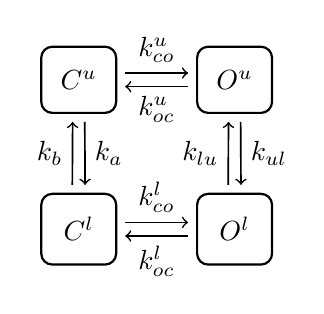
\begin{tikzpicture}[
   font=\sffamily,
   every matrix/.style={ampersand replacement=\&,column sep=1cm,row sep=1cm},
   state/.style={draw,thick,rounded corners,inner sep=.3cm},
   to/.style={->,semithick,shorten >=0.1cm,shorten <=0.1cm},
   Q/.style={->,semithick,sloped,pos=0.700000,shorten >=0.1cm,shorten <=0.1cm}, 
   every node/.style={auto}]
\matrix{
\node[state] (C^{u}) {\parbox{10pt}{\centerline{$C^{u}$}}};\&\node[state] (O^{u}) {\parbox{10pt}{\centerline{$O^{u}$}}};\\
\node[state] (C^{l}) {\parbox{10pt}{\centerline{$C^{l}$}}};\&\node[state] (O^{l}) {\parbox{10pt}{\centerline{$O^{l}$}}};\\
};
\draw[to]  (C^{u}.10) to node {$k_{co}^{u}$} (O^{u}.170);
\draw[to]  (C^{u}.280) to node {$k_{a}$} (C^{l}.80);
\draw[to]  (O^{u}.190) to node {$k_{oc}^{u}$} (C^{u}.350);
\draw[to]  (O^{u}.280) to node {$k_{ul}$} (O^{l}.80);
\draw[to]  (C^{l}.100) to node {$k_{b}$} (C^{u}.260);
\draw[to]  (C^{l}.10) to node {$k_{co}^{l}$} (O^{l}.170);
\draw[to]  (O^{l}.100) to node {$k_{lu}$} (O^{u}.260);
\draw[to]  (O^{l}.190) to node {$k_{oc}^{l}$} (C^{l}.350);
\end{tikzpicture}
\end{center}
\caption{Markov model with two open states ($O^{u}$, $O^{l}$) and two closed states ($C^{u}$, $C^{l}$).}
\label{o2}
\end{figure}
Assuming that the rates are set according to the principle of detailed balance,
 we have
\[k_{ul}o_{u}=k_{lu}o_{l}, \]
where $o_{u}$ and $o_{l}$ are the probabilities of being in the states 
$O^{u}$ or $O^{l}$, respectively, and $u$ and $l$ represent the upper and lower states,
respectively. 

As for the derivation above, we assume that the channel is open and
our task is to figure out how long we can expect the channel to remain open. We
know that, initially, the channel is either in the state $O^{u}$ or
$O^{l}$. Let us define $q_u$ and $q_l$ to be the conditional 
probabilities of being in the upper and lower open states, given that the channel is open. For the upper state we write
\[ q_u = P(S=O_u | (S={O_u} \mbox{\ or\ } S={O_l})), \]
where $S=X$ means that the channel is in state $X$.
Since
\[ P(A|B) = P(A \mbox{\ and\ } B)/P(B) \]
 and, in our case, since ($A$ and $B$) = $A$, we obtain
\[ q_u = P(S=O_u)/P(S={O_u} \mbox{\ or\ } S={O_l}) = \frac{o_u}{o_u+o_l} \]
and similarly for the lower state; with
\[ q_l = P(S=O_l | (S={O_u} \mbox{\ or\ } S={O_l})), \]
we obtain
\[ q_l  = \frac{o_l}{o_u+o_l}.\]
It follows that $q_u + q_l = 1$ and that

\[
q_{u}=\frac{k_{lu}}{k_{ul}+k_{lu}}
\]
and
\[
q_{l}=\frac{k_{ul}}{k_{ul}+k_{lu}}.
\]
The probability of remaining in the open states in the first time step is now given
by
\begin{align*}
p_{1}  & =\left(  1-\Delta tk_{oc}^{u}\right)  q_{u}+\left(  1-\Delta
tk_{oc}^{l}\right)  q_{l}\\
& =1-\Delta t\left(  \frac{k_{oc}^{u}k_{lu}+k_{oc}^{l}k_{ul}}{k_{ul}+k_{lu}
}\right)  
\end{align*}
and thus, by following the steps above, we find that
\[
p_{n}=\left(  1-\Delta tK\right)  ^{n},
\]
where
\[
K=\frac{k_{oc}^{u}k_{lu}+k_{oc}^{l}k_{ul}}{k_{ul}+k_{lu}}.
\]
The probability of closing a channel that is in one of the open states during
a time step is given by
\[
\Delta tk_{oc}^{u}q_{u}+\Delta tk_{oc}^{l}q_{l}=\Delta tK
\]
and, therefore, the probability of closing a channel in a time step that has
remained open for $n$ time steps is given by
\[
\Delta tK\left(  1-\Delta tK\right)^{n}.
\]
We find  that the expected mean open time is given by
\begin{equation}
\tau_{o}=\frac{1}{K}=\frac{k_{ul}+k_{lu}}{k_{oc}^{u}k_{lu}+k_{oc}^{l}k_{ul}}. \label{tau_oo}
\end{equation}

\subsubsection{Special cases}

It is interesting to consider the formula  for the mean open time given 
by $(\ref{tau_oo})$ in two special cases. First, we assume that 
$k^u_{oc}=k^l_{oc}$  and we let $k_{oc}$ denote this common value. Then, by $(\ref{tau_oo})$, we have 
\begin{equation*}
\tau_{o}=\frac{1}{k_{oc}}
\end{equation*}
which is the same as we found for the two-state scheme above. Next consider the case of $k_{ul}=k_{lu}$  (and 
$k^u_{oc}\not=k^l_{oc}$). By $(\ref{tau_oo})$, we find 
\begin{equation}
\tau_{o}=\frac{1}{(k_{oc}^{u}+k_{oc}^{u})/2}. \label{tau_ooo}
\end{equation}


\section{Numerical experiments}

It is useful to have a look at the mean open time computed in specific
numerical experiments to determine how well it is represented by the theoretical
value derived above. Similarly, it is useful to consider how well the
theoretical equilibrium open probability represents the data we observe in
actual computations. In this section, we will present experiments that
hopefully clarify these matters.

\subsection{Mean open time and equilibrium open probability: Theoretical
values versus sample mean values}

Let us illustrate the result above by a few numerical experiments. We start by
considering the Markov model
\[
C\underset{k_{co}}{\overset{k_{oc}}{\leftrightarrows}}O,
\]
where we set $k_{co}=1$ ms$^{-1}$ and we let
\[
k_{oc}=\frac{1}{m}\text{ms}^{-1}
\]
for $m=1,...,100.$ For every value of $k_{oc},$ we run a simulation using the
Markov model for $T=10^{4}$ ms. The time instances when the channel changes
state are stored in the sequence $\left\{  t_{i}\right\}  _{i=0}^{N}$ and the
mean open time observed in the simulation is given by\footnote{The
index $s$ here is used to indicate {\it sample}, since these are values for a
specific computation and not the theoretical value computed above.}
\[
\tau_{o,s}=\frac{2}{N}\sum_{i}\left(  t_{i}-t_{i-1}\right)  _{o},
\]
where
\[
\left(  t_{i}-t_{i-1}\right)  _{o}=\left\{
\begin{array}
[c]{ll}
t_{i}-t_{i-1}\text{ } & \text{if the channel is open in this interval,}\\
0\text{ } & \text{if the channel is closed in this interval.}
\end{array}
\text{ }\right.
\]
With this notation we can also define the sample open probability by
\[
o_{s}=\frac{1}{T}\sum_{i}\left(  t_{i}-t_{i-1}\right)  _{o}.
\]
In Figure  \ref{MOT:mot} (left panel), we plot the sample mean open time 
$\tau_{o,s}$ and the theoretical mean open time given by
\begin{equation}
\tau_{o}=\frac{1}{k_{oc}} \label{mot2}
\end{equation}
as functions of $k_{oc}.$ We also plot (right panel) the sample open
probability $o_{s}$ and the theoretical equilibrium probability given by
\begin{equation}
o=\frac{1}{1+\frac{k_{oc}}{k_{co}}}. \label{mot3}
\end{equation}
In both plots, we see that the mean values computed in the simulations are
quite close to the theoretical values. If we increase the simulation time $T,$
these graphs converge toward the same value.

FIGURE: [fig/MOT_mot.pdf, width=500 frac=0.8] Mean open time (left) and open probability (right), with $k_{oc}=1/m$ ms$^{-1}$ and $k_{co}=1$ ms$^{-1}$. The sample
values (dashed lines) correspond well with the theoretical values (solid line). label{MOT:mot}
\subsection{The closed to open rate $k_{co}$ does not affect the mean open
time}

We have seen that, theoretically, according to (ref{mot2})
the mean open time $\tau_{o}$ is independent of the closed to open rate
$k_{co},$ but the open probability is affected as stated in $\left(
\ref{mot3}\right)  .$ This is illustrated in Figure \ref{MOT:mct}, where we use
$k_{oc}=1$ ms$^{-1}$ and $k_{co}=1/m$ ms$^{-1}$ 
and plot the mean open time (left panel) and the open
probability (right panel) as functions of $m.$

FIGURE: [fig/MOT_mct.pdf, width=500 frac=0.8] Mean open time (left) and open probability (right) with $k_{co}=1/m$ ms$^{-1}$ and $k_{oc}=1$ ms$^{-1}$. The mean open
time is not affected by changes in $k_{co}$. The sample values correspond well to 
the theoretical values. label{MOT:mct}
\subsection{The mean open time in the presence of two open states}
In Figure \ref{MOT:burst_mot}, we show the sample mean open time and the theoretical mean open time given by 
\begin{equation}
\tau_{o}=\frac{1}{K}=\frac{k_{ul}+k_{lu}}{k_{oc}^{u}k_{lu}+k_{oc}^{l}k_{ul}} 
\end{equation}
for the Markov model in Figure \ref{o2}. In the computations, we have used $k^l_{oc} = 1$ ms$^{-1}$, $k^u_{oc} = 10$ ms$^{-1}$, and $k_{lu}  = 0.001$ ms$^{-1}$ and $k_{ul}$ varies. The other parameters of the model do not affect the result, as long as detailed balance holds.
FIGURE: [fig/MOT_burst_mot.pdf, width=500 frac=0.8] Mean open time for a Markov model with two open states. label{MOT:burst_mot}
\subsection[Changing MOT affects the dynamics of the transmembrane potential]{Changing the mean open time affects the dynamics of the transmembrane potential}
%\K{zzz For meg virker det som at parametrene som i de tidligere kapitlene 
%har blitt kalt for $V_{Na}$ og lignende n\r{a} blir kalt for $E_{Na}$ og lignende.
%Hvis det er tilfellet, er det greit med to forskjellige notasjoner eller
%burde det brukes den samme notasjonen? I kapittel 12 ble de samme 
%parameterverdiene brukt, men da ble $g_{K}$ og $E_{K}$ kalt for $g_{L}$ og $V_{L}$.
%Er det meningen at dette skal v\ae re det samme eksempelet eller er dette et
%annet eksempel?}
%\A{I have changed all back to $V_{Na}$ and $V_{K}$.}
We consider the stochastic model of the transmembrane potential given by
\begin{equation}
v_{t}=g_{K}(V_{K}-v)+\gamma g_{Na}(V_{Na}-v) \label{mot_s_1},
\end{equation}
where $\gamma$ is a stochastic variable governed by the two-state Markov
model
\[
C\underset{k_{co}}{\overset{k_{oc}}{\leftrightarrows}}O.
\]
We use the parameters
\begin{align}
g_{K}  &  =\frac{1}{10}\text{ ms}^{-1},\text{ }g_{Na}=1\text{ ms}
^{-1}, \label{mmm_dta}\\
V_{K} &  =-85\text{ mV, }V_{Na}=45\text{ mV,}\nonumber
\end{align}
and compute solutions using the standard scheme
\begin{equation}
v_{n+1}=v_{n}-\Delta t\left(  g_{K}\left(  v_{n}-V_{K}\right)  +\gamma
_{n}g_{Na}(v_{n}-V_{Na}\right)  ), \label{mot_vs}
\end{equation}
where the time step is assumed to satisfy the condition
\begin{equation}
\Delta t<\frac{1}{g_{K}+g_{Na}}.
\end{equation}
Under this condition, we have seen above that, for solutions computed by
(ref{mot_s_1}) an invariant region is given by
\begin{equation}
\Omega=\left(  V_{K},V_{+}\right)  ,
\end{equation}
where
\[
V_{+}=\frac{g_{K}V_{K}+g_{Na}V_{Na}}{g_{K}+g_{Na}}.
\]
In Figure \ref{MOT:time}, we show numerical solutions of (ref{mot_s_1})
for
\[
k_{oc}=k_{co}=0.1\text{ ms}^{-1},1\text{ ms}^{-1}, 10\text{ ms}^{-1}, 100 \text{ ms}^{-1}.
\]
According to the considerations above, the equilibrium open probability is
given by
\[
o=\frac{1}{1+\frac{k_{oc}}{k_{co}}},
\]
which is constant for the four parameter sets used in Figure \ref{MOT:time}. The mean
open time, however, varies with $k_{oc}$ as
\[
\tau_{o}=\frac{1}{k_{oc}}.
\]
For the cases studied in Figure \ref{MOT:time}, the mean open times are 
10 ms, 1 ms, 1/10 ms, and 1/100 ms and we observe that the reduced mean open time greatly 
reduces the variations of the transmembrane potential.

FIGURE: [fig/MOT_time.pdf, width=500 frac=0.8] Simulations based on the numerical scheme (\ref{mot_vs}) with 
changing reaction rates for the Markov model.
From top to bottom, $k_{oc}=k_{co}=0.1\text{ ms}^{-1}$, $1 \text{ ms}^{-1}$, $10\text{ ms}^{-1}$, and $100 \text{ ms}^{-1}.$ 
Since $k_{oc}=k_{co}$ for all values, the open probability
is kept constant but the mean open time given by $1/k_{oc}$ is decreasing from top 
to bottom.  label{MOT:time}
\section[Changing MOT affects the PDFs]{Changing the mean open time affects the probability density functions}

The stationary version of the probability density system governing the states
of the Markov model
\[
C\underset{k_{co}}{\overset{k_{oc}}{\leftrightarrows}}O
\]
is given by

\begin{align}
\frac{\partial}{\partial v}\left(  a_{o}\rho_{o}\right)   &  =k_{co}\rho
_{c}-k_{oc}\rho_{o},\label{vpdf_mot}\\
\frac{\partial}{\partial v}\left(  a_{c}\rho_{c}\right)   &  =k_{oc}\rho
_{o}-k_{co}\rho_{c},\nonumber
\end{align}
where 
\begin{align}
a_{o}  &  =g_{K}(V_{K}-v)+g_{Na}(V_{Na}-v),\label{vflux_mot}\\
a_{c}  &  =g_{K}(V_{K}-v).\nonumber
\end{align}
The analytical solution of this problem is given by

\begin{align*}
\rho_{o}(v)  &  =Kg_{K}(V_{+}-v)^{\frac{k_{oc}}{g}-1}(v-V_{K})^{\frac{k_{co}
}{g_{K}}},\\
\rho_{c}(v)  &  =Kg(V_{+}-v)^{\frac{k_{oc}}{g}}(v-V_{K})^{\frac{k_{co}}{g_{K}}-1},
\end{align*}
%\K{zzz Det skal vel egentlig st\r{a} v der det st\r{a}r x i disse uttrykkene?
%Og blir det ikke $(v-V_{K})$ i stedet for $(V_{K}-v)$ 
%siden vi antar $v \in (V_{K},V_{+})$?}\A{ Changed according to K.}
where
\[
g=g_{Na}+g_{K}\text{, }V_{+}=\frac{g_{Na}V_{Na}+g_{K}V_{K}}{g_{Na}+g_{K}}
\]
%\K{zzz Denne E-en ble kalt for $V_{+}$ i forrige seksjon.}\A{ Changed according to K.}
and $K$ is chosen such that
\[
\int_{V_{K}}^{V_{+}}\rho_{o}+\rho_{c}=1,
\]
which is given by
\[
1/K=\frac{k_{co}+k_{oc}}{a+b} (V_+-V_K)^{(a+b)} B(a,b),
\]
with $a = k_{co}/g_{K}, b = k_{oc}/g$, and $B(a,b) =\Gamma(a)\Gamma(b)/\Gamma(a+b)$.
%\K{zzz Burde det st\r{a} $V_{K}$ i stedet for $V_{-}$ i uttrykket slik at det henger mer sammen med det over?}


In Figure \ref{MOT:pdf}, we show the open probability density function for the data given
in (ref{mmm_dta}) with
\[
k_{oc}=k_{co}=0.1 \text{ ms}^{-1},1\text{ ms}^{-1},10\text{ ms}^{-1},100 \text{ ms}^{-1}.
\]
Again, we recall that as $k_{oc}$ increases, the mean open time
decreases and we observe in the figure that the probability density function
becomes narrower.
%\K{zzz stoppet her}

FIGURE: [fig/MOT_pdf.pdf, width=500 frac=0.8] The open probability density function $\rho_o$ (solid line) and closed
 probability density function $\rho_c$ depend on the mean open time given by $1/k_{oc}$. In the figures,
 we have used $k=k_{oc}=k_{co}.$ label{MOT:pdf}\bigskip

\begin{comment}
\subsection{The limit of the zero mean open time}

In Figure \ref{MOT:pdf}, we observed that as $k_{oc}$ and $k_{co}$ increase, the open
probability density function becomes increasingly narrow and it is tempting to
understand where this ends. Let $k=k_{oc}=k_{co}$ and consider the probability
density system
\begin{align}
\frac{1}{k}\frac{\partial}{\partial v}\left(  a_{o}\rho_{o}\right)   &
=\rho_{c}-\rho_{o},\label{mot_k}\\
\frac{1}{k}\frac{\partial}{\partial v}\left(  a_{c}\rho_{c}\right)   &
=\rho_{o}-\rho_{c}.\nonumber
\end{align}
In the limit of $k\longrightarrow\infty,$ the mean open time
\[
\tau_{o}=\frac{1}{k_{oc}}=\frac{1}{k}\longrightarrow0
\]
and, by (\ref{mot_k}), we have
\[
\rho_{c}=\rho_{o}.
\]
By adding the equations, we obtain (for any value of $k$)
\[
\frac{\partial}{\partial v}\left(  a_{o}\rho_{o}+a_{c}\rho_{c}\right)  =0
\]
and with $\rho_{o}=\rho_{c},$ this yields
\[
\frac{\partial}{\partial v}\left(  \left(  a_{o}+a_{c}\right)  \rho
_{o}\right)  =0.
\]
Since $\rho_{o}=0$ for sufficiently large values of $\left\vert v\right\vert
,$ we find that
\begin{equation}
\left(  a_{o}+a_{c}\right)  \rho_{o}=0 \label{0}
\end{equation}
for almost all\footnote{This means {\sl almost all} in this sense: \url{http://en.wikipedia.org/wiki/Almost_all}.} $v$. Since
 $\rho_{o}=\rho_{c},$ we have
\[
\int\rho_{o}dv=\frac{1}{2}
\]
and thus $\rho_{o}=\frac{1}{2}\delta\left(  v-v_{\ast}\right)  , $ where
$\delta$ is the Dirac delta function. In general, we have
\[
\int f(v)\delta\left(  v-v_{\ast}\right)  dv=f\left(  v_{\ast}\right)
\]
and, therefore, by (\ref{0}), we must have
\[
\left(  a_{o}+a_{c}\right)  \left(  v_{\ast}\right)  =\frac{1}{2}\int\left(
a_{o}+a_{c}\right)  \left(  v\right)  \delta\left(  v-v_{\ast}\right)
dv=0.
\]
By using the definitions (ref{vflux_mot}), we obtain
\[
2g_{K}(V_{K}-v_{\ast})+g_{Na}(V_{Na}-v_{\ast})=0
\]
and therefore
\[
v_{\ast}=\frac{2g_{K}V_{K}+g_{Na}V_{Na}}{2g_{K}+g_{Na}}.
\]
In Figure \ref{MOT:pdf} we show the open and closed probability density functions
defined by the system (ref{mot_k}) We observe that as $k$
increases, the functions converges and the distributions center around
$v_{\ast}=23.33$ mV. In these computations we have used the parameters defined in (\ref{mmm_dta}).

{\bf xxx Glenn: Kan du legge inn stoerre verdier av $k$ slik at vi ser at 
peak-verdier  konvergerer mot $v^*$?}
\G{Updated parameter value in text, peak should be at $v_{\ast}=23.33.$, so the plots are OK as is I guess.}

\end{comment}


\section{Theoretical drugs for OC-mutations}

We have seen earlier that when mutations increase the open probability by
increasing the reaction rate from C to O $(k_{co}),$ the effect of the
mutation can be completely repaired by using an optimal closed state blocker.
Now we are interested in a mutation that increases the open probability by reducing
the reaction rate from O to C $\left(  k_{oc}\right).$ Such a mutation
increases both the open probability and  the mean open time
and we will observe that a closed state blocker is unable to repair the effect
of such a mutation.

We consider the two-state Markov model
\begin{equation}
C\underset{k_{co}}{\overset{k_{oc}/\mu}{\leftrightarrows}}O, \label{mmm0}
\end{equation}
where $\mu\geqslant1$ is the mutation severity index; as usual, $\mu=1$ denotes
the wild type. Recall that the equilibrium open probability is given by
\[
o=\frac{1}{1+\frac{k_{oc}}{\mu k_{co}}}
\]
and the mean open time is given by
\[
\tau_{o}=\frac{\mu}{k_{oc}},
\]
so the mutation clearly increases both the open probability and the mean open time.

\bigskip

\subsection{The theoretical closed state blocker does not work for the OC-mutation}

Let us start by considering a closed state blocker of the form
\begin{equation}
B\underset{k_{bc}}{\overset{k_{cb}}{\leftrightarrows}}C\underset{k_{co}}{\overset{k_{oc}/\mu}{\leftrightarrows}}O. \label{mmm1}
\end{equation}
%\K{zzz Burde man i denne Markov-modellen heller ta med at vi deler $k_{oc}$ 
%p\r{a} $\mu$?}
% A: ja; fixet
We find that the equilibrium open probability of the mutant in the presence of the
closed state blocker is given by
\[
o=\frac{1}{1+\frac{k_{oc}}{k_{co}}\frac{1+\delta_{c}}{\mu}},
\]
where
\[
\delta_{c}=\frac{k_{cb}}{k_{bc}}.
\]
Since the wild type equilibrium open probability is given by
\[
o=\frac{1}{1+\frac{k_{oc}}{k_{co}}},
\]
the drug will repair the open probability, provided that
\[
\frac{1+\delta_{c}}{\mu}=1
\]
and therefore the drug must satisfy the usual condition
\[
\delta_{c}=\mu-1.
\]
A drug satisfying this condition will completely repair the equilibrium open
probability and that is, of course, good, but it is not enough. Since the
mutation represented by (ref{mmm0}) also affects the mean
open time, a drug of the form (ref{mmm1}) cannot repair that
effect of the mutation. To see this, we consider the probability
density system defined by
\begin{align}
\frac{\partial}{\partial v}\left(  a_{o}\rho_{o}\right)   &  =k_{co}\rho
_{c}-\frac{1}{\mu}k_{oc}\rho_{o},\nonumber\\
\frac{\partial}{\partial v}\left(  a_{c}\rho_{c}\right)   &  =\frac{1}{\mu}k_{oc}\rho
_{o}-\left(  k_{co}+\left(  \mu-1\right)  k_{bc}\right)  \rho_{c}+k_{bc}
\rho_{b},\label{mmm3}\\
\frac{\partial}{\partial v}\left(  a_{c}\rho_{b}\right)   &  =\left(
\mu-1\right)  k_{bc}\rho_{c}-k_{bc}\rho_{b},\nonumber
\end{align}
%\K{zzz Skal man ikke i disse ligningene dele $k_{oc}$ p\r{a} $\mu$?}
where, as usual, $\rho_{o},\rho_{c},$ and $\rho_{b}$ denote the probability
density functions of the open (O), closed (C), and blocked (B) states,
respectively, and where the fluxes are defined by $\left(  \ref{vflux_mot}
\right)  $. In Figure \ref{MOT:cb}, we compare the open probability density computed by
solving the system (ref{mmm3}) with the open probability
density of the wild type. The wild type probability density functions are
given by

\begin{align}
\frac{\partial}{\partial v}\left(  a_{o}\rho_{o}\right)   &  =k_{co}\rho
_{c}-k_{oc}\rho_{o},\label{mmm4}\\
\frac{\partial}{\partial v}\left(  a_{c}\rho_{c}\right)   &  =k_{oc}\rho
_{o}-k_{co}\rho_{c},\nonumber
\end{align}
and the probability density functions of the mutant case are given by
\begin{align}
\frac{\partial}{\partial v}\left(  a_{o}\rho_{o}\right)   &  =k_{co}\rho
_{c}-\frac{1}{\mu}k_{oc}\rho_{o},\label{mutant44}\\
\frac{\partial}{\partial v}\left(  a_{c}\rho_{c}\right)   &  =\frac{1}{\mu}k_{oc}\rho
_{o}-k_{co}\rho_{c}.\nonumber
\end{align}
In the computations we have used the parameters given by $\left(
\ref{mmm_dta}\right)  $ and the rates
\[
k_{co}=1\text{ ms}^{-1} \text{ and }k_{oc}=1\text{ ms}^{-1}.
\]
We use three values of the rates $k_{bc}$ and we observe that no parameter is
able to repair the open state probability density function of the mutation. In
Figure \ref{MOT:norm}, we show the norm of the difference between the open probability
density defined by (ref{mmm3}) and $\left(  \ref{mmm4}
\right)  .$ The norm is defined by (ref{norm}) on page
\pageref{norm} and we see that no version of the closed state blocker defined 
by (ref{mmm1}) is able to repair the effect of the mutations
given by (ref{mmm0})

FIGURE: [fig/MOT_cb.pdf, width=500 frac=0.8] The solid line represents the wild type solution and the dashed line represents the mutant. Various closed state drugs are applied, but none are able to repair the effect of the mutation. label{MOT:cb}FIGURE: [fig/MOT_norm.pdf, width=500 frac=0.8] The norm of the difference between the wild type solution and the mutant after the drug is applied. 
The norm is defined by (ref{norm}) on page \pageref{norm}. We see that no value of the drug parameter 
$k_{bc}$ for the closed state blocker is able to repair the effect of the mutation.
 label{MOT:norm}
\subsection{The theoretical open state blocker repairs the effect of the OC-mutation}

Next, we consider an open state blocker for the mutation leading to both an
increased open probability and an increased mean open time. The theoretical open 
state blocker can be written in the form
\begin{equation}
C\underset{k_{co}}{\overset{k_{oc}/\mu}{\leftrightarrows}}O\underset{k_{ob}
}{\overset{k_{bo}}{\leftrightarrows}}B, \label{mmob1}
\end{equation}
where the parameters $k_{bo}$ and $k_{ob}$ define the theoretical drug. For this
Markov model, the equilibrium open probability is given by
\[
o_{\mu}=\frac{1}{1+\frac{k_{oc}}{\mu k_{co}}+\frac{k_{ob}}{k_{bo}}}
\]
and the mean open time is given by
\[
\tau_{o,\mu}=\frac{1}{\frac{1}{\mu}k_{oc}+k_{ob}}.
\]
Since the associated wild type values are
\[
o=\frac{1}{1+\frac{k_{oc}}{k_{co}}}
\]
and
\[
\tau_{o}=\frac{1}{k_{oc}},
\]
we want to define the drug such that
\[
1+\frac{k_{oc}}{\mu k_{co}}+\frac{k_{ob}}{k_{bo}}=1+\frac{k_{oc}}{k_{co}}
\]
and
\[
\frac{1}{\mu}k_{oc}+k_{ob}=k_{oc}.
\]
To satisfy these two requirements, we find that the drug must be given by
\begin{equation} \label{mot_o_drg}
\begin{aligned}
k_{ob}  &  =\frac{\mu-1}{\mu}k_{oc},\\
k_{bo}  &  =k_{co}.
\end{aligned}
\end{equation}

\subsection{The theoretical open state blocker is optimal}
We will show analytically that the open state blocker defined by (\ref{mmob1}) where the parameters are given by
(\ref{mot_o_drg}) is an optimal drug, in the sense that the effect of the mutation is completely repaired.
We start by observing that the probability density system associated with the Markov model  (\ref{mmob1}) is given by
\begin{align}
\frac{\partial}{\partial v}\left(  a_{o}\rho_{o}\right)   &  =k_{co}\rho
_{c}-(\mu^{-1}k_{oc}+k_{ob})\rho_{o}+k_{bo}\rho_{b},\nonumber\\
\frac{\partial}{\partial v}\left(  a_{c}\rho_{c}\right)   &  =\mu^{-1}
k_{oc}\rho_{o}-k_{co}\rho_{c},\label{mm_dr_3}\\
\frac{\partial}{\partial v}\left(  a_{c}\rho_{b}\right)   &  =k_{ob}\rho
_{o}-k_{bo}\rho_{b}.\nonumber
\end{align}
If we insert the drug given by (ref{mot_o_drg}), we obtain the
system
\begin{align}
\frac{\partial}{\partial v}\left(  a_{o}\rho_{o}\right)   &  =k_{co}\rho
_{c}-k_{oc}\rho_{o}+k_{co}\rho_{b},\nonumber\\
\frac{\partial}{\partial v}\left(  a_{c}\rho_{c}\right)   &  =\mu^{-1}
k_{oc}\rho_{o}-k_{co}\rho_{c},\label{mm_dr_o2}\\
\frac{\partial}{\partial v}\left(  a_{c}\rho_{b}\right)   &  =\left(
1-\mu^{-1}\right)  k_{oc}\rho_{o}-k_{co}\rho_{b}.\nonumber
\end{align}
We define
\[
\bar{\rho}_{c}=\rho_{c}+\rho_{b}
\]
and add the two latter equations of this system to find that $\rho_{o}$ and 
$\bar{\rho}_{c}$ solve the system
\begin{align}
\frac{\partial}{\partial v}\left(  a_{o}\rho_{o}\right)   &  =k_{co}\bar{\rho
}_{c}-k_{oc}\rho_{o},\\
\frac{\partial}{\partial v}\left(  a_{c}\bar{\rho}_{c}\right)   &  =k_{oc}
\rho_{o}-k_{co}\bar{\rho}_{c},\nonumber
\end{align}
which coincides with the system defining the wild type probability density
functions (see (ref{mmm4}) above). We therefore conclude that
the open state blocker defined by the parameters 
(ref{mot_o_drg})
completely repairs the probability density functions of the mutant for any
value of the mutation severity index.

\bigskip

\subsubsection{The probability density function of the blocked state is
proportional to the probability density function of the wild type closed state}


In Figure \ref{MOT:ob}, we show the open probability density functions of the
wild type
(defined by system (ref{mmm4}) the mutant (defined by system (ref{mutant44}) with $\mu=3),$ 
%\K{zzz (\ref{mmm3}) er ligningene for closed state blocker. 
%Tror ikke at ligningene for mutant uten drug st\r{a}r noe sted.} 
and the mutant including the optimal drug (defined by system 
(ref{mm_dr_o2}) As expected, the open probability is 
completely repaired by the theoretical drug.

In the right panel of the figure, we show the graph of $\rho_{c}$ for the wild type
(solid line) and for the mutant case in the presence of the open blocker. We show
both $\rho_{c}$ and $\rho_{b}$. We note that these graphs seem to have the same 
shape  and we will show that they indeed differ only by a constant. 

We start by making the ansatz that for the solution of system (ref{mm_dr_o2}) we have
\begin{equation}
\rho_{b}=\left(  \mu-1\right)  \rho_{c}. \label{mot_ans}
\end{equation}
If we insert this into system (ref{mm_dr_o2}), we find that
the two latter equations become identical and the system is therefore reduced to the following $2\times 2$
system:
\begin{align}
\frac{\partial}{\partial v}\left(  a_{o}\rho_{o}\right)   &  =\mu k_{co}
\rho_{c}-k_{oc}\rho_{o},\nonumber\\
\frac{\partial}{\partial v}\left(  a_{c}\rho_{c}\right)   &  =\mu^{-1}
k_{oc}\rho_{o}-k_{co}\rho_{c}.
\end{align}
Therefore, we can define
\[
\rho_{c}^{\ast}=\mu\rho_{c}
\]
and find that $\rho_{o}$ and $\rho_{c}^{\ast}$ solve system
\begin{align}
\frac{\partial}{\partial v}\left(  a_{o}\rho_{o}\right)   &  = k_{co}
\rho_{c}^{\ast}-k_{oc}\rho_{o},\nonumber\\
\frac{\partial}{\partial v}\left(  a_{c}\rho_{c}^{\ast}\right)   &
=k_{oc}\rho_{o}-k_{co}\rho_{c}^{\ast},
\end{align}
which is exactly the wild type system. We therefore conclude that 
\begin{equation}
\rho_{b}=\left(  \mu-1\right)  \rho_{c}=\frac{\mu-1}{\mu}  \rho^*_{c}, \label{rb}
\end{equation}
where $(\rho_{o},\rho_{c},\rho_{b})$ solves the system (ref{mm_dr_o2})
and where $(\rho^*_{o},\rho^*_{c})$ solves the wild type system
\begin{align*}
\frac{\partial}{\partial v}\left(  a_{o}\rho^*_{o}\right)   &  =k_{co}\rho^*_{c}-k_{oc}\rho^*_{o},\\
\frac{\partial}{\partial v}\left(  a_{c}\rho^*_{c}\right)   &  =k_{oc}
\rho^*_{o}-k_{co}\rho^*_{c}.
\end{align*}

%{\bf Glenn: Can you check you numerical results and see if I have got the constant right; check the correctness
%of (\ref{rb}) by a numerical comparison.}
%\G{The ratios in Fig 13.9 are spot on (1/3 and 2/3).}
FIGURE: [fig/MOT_ob.pdf, width=500 frac=0.8] Probability density functions of the wild type, mutant, and mutant in the presence of the open blocker. The open blocker completely
repairs the open probability density function of the mutant.  label{MOT:ob}
%\bf xxx Glenn: Is there something wrong in the right panel? In the
%left panel the two first curves are $\rho_o$ for wt and mt; but in the right panel it is
%$\rho_c$ for wt and

\subsection{Stochastic simulations using the optimal open state blocker}

In Figure \ref{MOT:ob_mc}, we show the results of numerical
simulations using scheme
(ref{mot_vs}) We show the result for the wild type model
(upper panel), the mutant model (middle panel), and the model of the mutant 
where the drug defined by (ref{mot_o_drg}) is used (lower panel).

The graphs show that the effect of the mutation is repaired using the drug $\left(
\ref{mot_o_drg}\right) $; the solutions are not identical and this is
reasonable, since a random number generator is involved in updating the state
of the Markov model and therefore two computed solutions will not be identical
(not even two wild type solutions). However, we note that the qualitative properties
of the upper and lower solutions are similar, whereas the mutant case is
different due to the increased open probability and prolonged mean open time.

FIGURE: [fig/MOT_ob_mc.pdf, width=500 frac=0.8] Numerical simulations using scheme (ref{mot_vs})
for wild type data (upper panel), mutant data (center panel), and mutant data where the drug
defined by (ref{mot_o_drg}) is used (lower panel). 
Observe the long open periods in the middle panel
and that these are repaired by the drug (lower panel). label{MOT:ob_mc}\section{Inactivated states and mean open time}

In Chapter \ref{inactivated}, we studied a Markov model including the
open state (O), closed state (C), and inactivated state (I). The prototypical 
Markov model is repeated in Figure \ref{MOT_mut_L:ICO}.
 As usual, we assumed that the principle of detailed balance holds and
therefore the parameters of the Markov model satisfy the equation
\begin{equation}
k_{io}k_{oc}k_{ci}=k_{oi}k_{co}k_{ic}.\label{db_m}
\end{equation}
We also introduced a mutation that increased the rates $k_{io}$ and $k_{ic}$ and thus
reduced the probability of being in the inactivated state. From what we have
just seen, we readily observe that such a mutation does not influence the mean
open time; however, if data show that the mean open time is affected, the effect of
the mutation must be modeled differently. Another way to model the reduced
equilibrium probability of being in the inactivated state is to reduce the
rates toward the inactivated state. Such a mutation takes the form
\begin{align}
\bar{k}_{ci} &  =k_{ci}/\mu,\label{ratesvm_m}\\
\bar{k}_{oi} &  =k_{oi}/\mu, \nonumber
\end{align}
where $\mu\geqslant1$ and, as usual, $\mu=1$ represents the wild type. It
follows from (ref{db_m}) that the principle of detailed
balance also holds for the mutant model:
\begin{equation}
k_{io}k_{oc}\frac{k_{ci}}{\mu}=\frac{k_{oi}}{\mu}k_{co}k_{ic}.\label{db_mm}
\end{equation}
If we repeat the argument above, we find that the mean open time of the model
presented in Figure \ref{MOT_mut_L:ICO} is given by
\[
\tau_{o}=\frac{1}{k_{oc}+k_{oi}}% 
\]
for wild type data and
\[
\tau_{o,\mu}=\frac{1}{k_{oc}+k_{oi}/\mu}
\]
for the mutant case. We note that the mean open time increases as the mutation severity
index $\mu$ increases. Following the usual steps, we find that the equilibrium
probabilities are given by
\begin{align*}
o &  =\frac{1}{1+\frac{k_{oc}}{k_{co}}+\frac{k_{oi}}{\mu k_{io}}},\\
c &  =\frac{\frac{k_{oc}}{k_{co}}}{1+\frac{k_{oc}}{k_{co}}+\frac{k_{oi}}{\mu
k_{io}}},\\
i &  =\frac{\frac{k_{oi}}{k_{io}}}{\mu\left(  1+\frac{k_{oc}}{k_{co}}\right)
+\frac{k_{oi}}{k_{io}}}.
\end{align*}
We observe that the equilibrium probability of being in the open and closed states
increases as a consequence of the mutation and the equilibrium probability of
being in the inactivated state is reduced under the mutation.

\begin{figure}[ptb]
\begin{center}
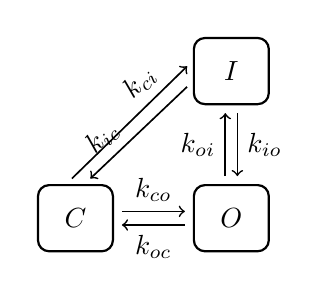
\begin{tikzpicture}[
   font=\sffamily,
   every matrix/.style={ampersand replacement=\&,column sep=1cm,row sep=1cm},
   state/.style={draw,thick,rounded corners,inner sep=.3cm},
   to/.style={->,semithick,shorten >=0.1cm,shorten <=0.1cm},
   Q/.style={->,semithick,sloped,pos=0.700000,shorten >=0.1cm,shorten <=0.1cm}, 
   every node/.style={auto}]
\matrix{
\&\node[state] (I) {\parbox{10pt}{\centerline{$I$}}};\\
\node[state] (C) {\parbox{10pt}{\centerline{$C$}}};\&\node[state] (O) {\parbox{10pt}{\centerline{$O$}}};\\
};
\draw[to]  (O.100) to node {$k_{oi}$} (I.260);
\draw[to]  (O.190) to node {$k_{oc}$} (C.350);
\draw[to]  (I.280) to node {$k_{io}$} (O.80);
\draw[Q]  (I.195) to node {$k_{ic}$} (C.75);
\draw[to]  (C.10) to node {$k_{co}$} (O.170);
\draw[Q]  (C.105) to node {$k_{ci}$} (I.165);
\end{tikzpicture}
\end{center}
\caption{Three-state Markov model. In the mutant case, we
replace the rates $k_{ci}$ and $k_{oi}$ by  $k_{ci}/\mu$ and $k_{oi}/\mu$, 
respectively, where $\mu$ denotes the mutation severity index.}
\label{MOT_mut_L:ICO}
\end{figure}


%FIGURE: [fig/MOT_mut_L_ICO.pdf, width=500 frac=0.8] Three state Markov model. In the mutant case we
%replace the rates $k_{ci}$ and $k_{oi}$ by  $k_{ci}/\mu$ and $k_{oi}/\mu$ where
%$\mu$ denotes the mutation severity index. label{MOT_mut_L:ICO}

\subsection{A theoretical open state blocker}



We observed above that to repair the effect of changes in the mean
open time, it is necessary to use an open state blocker. The reason for this is 
that neither a closed blocker nor an inactivated blocker has any effect on the 
mean open time and, therefore, it is inconceivable that such blockers 
can repair the effect of a mutation on the mean open time. An open state blocker 
directly affects the mean open time and the drug must be tuned to repair the 
effect of the mutation.

A Markov model that includes an open state blocker is shown in 
Figure \ref{MOT_mut_L:BICO_O}.
We have already computed
formulas for the equilibrium probabilities of a Markov model of this form (see
page \pageref{Ionchannels_L:BICO}). The inverse $(p=1/o)$ open probability in equilibrium is given by
\[
p_{\mu}=1+\frac{k_{oc}}{k_{co}}+\frac{1}{\mu}\frac{k_{oi}}{k_{io}}
\]
and thus the wild type inverse open probability is given by
\[
p=1+\frac{k_{oc}}{k_{co}}+\frac{k_{oi}}{k_{io}}.
\]
Similarly, the inverse open probability in the presence of the open state blocker 
is given by
\[
p_{b,\mu}=1+\frac{k_{oc}}{k_{co}}+\frac{1}{\mu}\frac{k_{oi}}{k_{io}}+\frac{k_{ob}
}{k_{bo}}.
\]
Furthermore, the mean open time of wild type is given by
\[
\tau_{o}=\frac{1}{k_{oi}+k_{oc}}
\]
and, when the theoretical drug is included in the mutant case, the mean open
time is given by
\[
\tau_{o,b,\mu}=\frac{1}{\frac{1}{\mu}k_{oi}+k_{oc}+k_{ob}}.
\]
We are now looking for a drug that will repair the equilibrium probability and
the mean open time. More precisely, we want to find the parameters $k_{bo}$
and $k_{ob}$ such that $p_{b,\mu}=p$ and $\tau_{o,b,\mu}=\tau_{o}$. More explicitly, we require that
\[
1+\frac{k_{oc}}{k_{co}}+\frac{1}{\mu}\frac{k_{oi}}{k_{io}}+\frac{k_{ob}
}{k_{bo}}=1+\frac{k_{oc}}{k_{co}}+\frac{k_{oi}}{k_{io}}\text{ }
\]
and
\[
\frac{1}{\mu}k_{oi}+k_{oc}+k_{ob}=k_{oi}+k_{oc}.
\]
This is a $2\times 2$ system of equations in the unknowns $k_{ob}$ and $k_{bo}$ and the 
solution is given by
\begin{equation}
k_{ob}=\left(  1-\mu^{-1}\right)  k_{oi}\text{ and }k_{bo}=k_{io}.\label{mot_in_dr}
\end{equation}
We will see in numerical experiments below that the open state blocker
illustrated in Figure  \ref{MOT_mut_L:BICO_O} where the parameters of the drug are given by (\ref{mot_in_dr})
repairs the effect of the mutation.

\begin{figure}[ptb]
\begin{center}
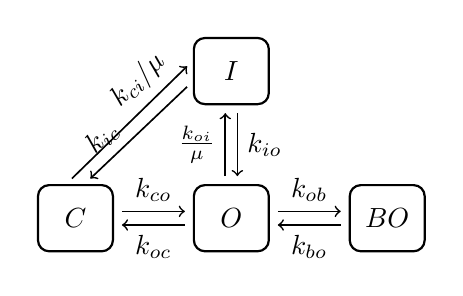
\begin{tikzpicture}[
   font=\sffamily,
   every matrix/.style={ampersand replacement=\&,column sep=1cm,row sep=1cm},
   state/.style={draw,thick,rounded corners,inner sep=.3cm},
   to/.style={->,semithick,shorten >=0.1cm,shorten <=0.1cm},
   Q/.style={->,semithick,sloped,pos=0.700000,shorten >=0.1cm,shorten <=0.1cm},  
   every node/.style={auto}]
\matrix{
\&\node[state] (I) {\parbox{10pt}{\centerline{$I$}}};\&\\
\node[state] (C) {\parbox{10pt}{\centerline{$C$}}};\&\node[state] (O) {\parbox{10pt}{\centerline{$O$}}};\&\node[state] (BO) {\parbox{10pt}{\centerline{$BO$}}};\\
};
\draw[to]  (O.100) to node {$\frac{k_{oi}}{\mu}$} (I.260);
\draw[to]  (O.190) to node {$k_{oc}$} (C.350);
\draw[to]  (O.10) to node {$k_{ob}$} (BO.170);
\draw[to]  (I.280) to node {$k_{io}$} (O.80);
\draw[Q]  (I.195) to node {$k_{ic}$} (C.75);
\draw[to]  (C.10) to node {$k_{co}$} (O.170);
\draw[Q]  (C.105) to node {$k_{ci}/\mu$} (I.165);
\draw[to]  (BO.190) to node {$k_{bo}$} (O.350);
\end{tikzpicture}
\end{center}
\caption{The model represented in Figure  \ref{MOT_mut_L:ICO} is extended 
to account for the blocker (BO) associated with the open state.}
\label{MOT_mut_L:BICO_O}
\end{figure}

%FIGURE: [fig/MOT_mut_L_BICO_O.pdf, width=500 frac=0.8] The model represented in Figure  \ref{MOT_mut_L:ICO} extended to account for
%the blocker (BO) associated the open state. label{MOT_mut_L:BICO_O}
\subsection{Probability density functions using the open state blocker}

We have found a theoretical drug (see (ref{mot_in_dr})) for
the mutation affecting the rates from O to I and from C to I and we want to
assess the drug's usefulness by considering the open probability density
functions. For the wild type case, the probability density functions of the
states present in the Markov model of Figure \ref{MOT_mut_L:ICO} are
governed by the system


\begin{align}
\frac{\partial}{\partial v}\left(  a_{o}\rho_{o}\right)   &  =k_{co}\rho
_{c}-\left(  k_{oc}+k_{oi}\right)  \rho_{o}+k_{io}\rho_{i},\nonumber\\
\frac{\partial}{\partial v}\left(  a_{c}\rho_{c}\right)   &  =k_{oc}\rho
_{o}-\left(  k_{co}+k_{ci}\right)  \rho_{c}+k_{ic}\rho_{i},\label{wt_mt_in}\\
\frac{\partial}{\partial v}\left(  a_{c}\rho_{i}\right)   &  =k_{oi}\rho
_{o}-(k_{io}+k_{ic})\rho_{i}+k_{ci}\rho_{c}.\nonumber
\end{align}
In the mutant case, when the open state blocker is added as indicated in Figure
\ref{MOT_mut_L:BICO_O}, the probability density system is
\begin{align}
\frac{\partial}{\partial v}\left(  a_{o}\rho_{o}\right)   &  =k_{co}\rho
_{c}-\left(  k_{oc}+\frac{1}{\mu}k_{oi}+k_{ob}\right)  \rho_{o}+k_{io}\rho_{i}
+k_{bo}\rho_{b},\nonumber\\
\frac{\partial}{\partial v}\left(  a_{c}\rho_{c}\right)   &  =k_{oc}\rho
_{o}-\left(  k_{co}+\frac{1}{\mu}k_{ci}\right)  \rho_{c}+k_{ic}\rho
_{i},\label{mot_dr_123}\\
\frac{\partial}{\partial v}\left(  a_{c}\rho_{i}\right)   &  =\frac{1}{\mu
}k_{oi}\rho_{o}-(k_{io}+k_{ic})\rho_{i}+\frac{1}{\mu}k_{ci}\rho_{c}
,\nonumber\\
\frac{\partial}{\partial v}\left(  a_{c}\rho_{b}\right)   &  =k_{ob}\rho
_{o}-k_{bo}\rho_{b}.\nonumber
\end{align}
%\K{zzz Skal man ikke i den f\o rste ligningen  i (\ref{mot_dr_123}) ha med leddet $-k_{ob}\rho_{o}$? I s\r{a} fall m\r{a} man vel ogs\r{a} endre fra  $\left(  k_{oc}+\frac{1}{\mu}k_{oi}\right)  \rho_{o}$ til $\left(  k_{oc}+k_{oi}\right)  \rho_{o}$ i den f\o rste ligningen i (\ref{mot_dr_124})?}
%{\bf xxx Glenn: I have corrected the text according to Karoline; can you check the code?}
%\G{This was correct in the code. In general, models are implemented based on the  figure, not the math. (And diagonal entries are computed automatically.)}
As usual, $\rho_{o},\rho_{c},\rho_{i},$ and $\rho_{b}$ denote the probability density
functions of the open, closed, inactivated, and blocked states, respectively,
and the functions of the flux are given by (ref{vflux_mot}) By introducing
the drug given by (ref{mot_in_dr}), we obtain the system
\begin{align}
\frac{\partial}{\partial v}\left(  a_{o}\rho_{o}\right)   &  =k_{co}\rho
_{c}-\left(  k_{oc}+k_{oi}\right)  \rho_{o}+k_{io}\rho_{i}
+k_{io}\rho_{b},\nonumber\\
\frac{\partial}{\partial v}\left(  a_{c}\rho_{c}\right)   &  =k_{oc}\rho
_{o}-\left(  k_{co}+\frac{1}{\mu}k_{ci}\right)  \rho_{c}+k_{ic}\rho
_{i},\label{mot_dr_124}\\
\frac{\partial}{\partial v}\left(  a_{c}\rho_{i}\right)   &  =\frac{1}{\mu
}k_{oi}\rho_{o}-(k_{io}+k_{ic})\rho_{i}+\frac{1}{\mu}k_{ci}\rho_{c}
,\nonumber\\
\frac{\partial}{\partial v}\left(  a_{c}\rho_{b}\right)   &  =\left(
1-\mu^{-1}\right)  k_{oi}\rho_{o}-k_{io}\rho_{b}.\nonumber
\end{align}
In Figure \ref{MOT:iocb}, we show solutions of the wild type system 
(ref{wt_mt_in}), the mutant system, and the mutant system where the
drug is added (ref{mot_dr_124}). Note that the mutant system
is equal to the wild type system, except for the change of the rates $k_{ci}$
and $k_{oi}$ given by
\begin{align}
\bar{k}_{ci} &  =k_{ci}/\mu,\\
\bar{k}_{oi} &  =k_{oi}/\mu.\nonumber
\end{align}
In Figure \ref{MOT:iocb},  we compare the open probability density functions of the three models for three
different sets of parameters. In the left panel of Figure \ref{MOT:iocb},  we show the open probability of the wild type (solid line),
 the mutant ($\mu=10$), and the mutant in the presence of the theoretical open blocker. We see that the effect of the
 mutation is completely repaired by the drug. Other cases are shown in the center and right panels. The effect of the drug is still good but the effect of the mutation is not completely repaired. These observations are confirmed in Table \ref{tab:iocb}.
Furthermore, we have  tested a large variety of parameters and the results 
we show here (center and right panels)  represent the most difficult cases we could find in experiments. 
Therefore, we conclude that the theoretical open state blocker illustrated in Figure  \ref{MOT_mut_L:BICO_O}
 works very well. 

FIGURE: [fig/MOT_iocb.pdf, width=500 frac=0.8] Left panel: All rates equal one. The theoretical drug restores $\rho_o$. Middle panel: As in the left panel, except $k_{co}=10\text{ ms}^{-1}$. 
Right panel:  As in the left panel, except $k_{io}=0.1\text{ ms}^{-1}$. For all three cases, $\mu = 10$.}
%\G{Jeg har testet hver parameter for seg, fra 0.01 til 100. Det er kun disse parameterne som kan gi betydelige avvik, og det blir ikke verre en det vises her, som jo egentlig er ganske bra.}} 

%{\bf xxx Glenn: Can you compute the usual statistical properties of the three cases of 
%Figure \ref{MOT_mut_L:BICO_O} and put it in a table?}
%\G{This is now Table \ref{tab:iocb} label{MOT:iocb}\begin{table}  \begin{center}
\begin{tabular}{|c|r|r|r|r|r|r|} \hline
& \multicolumn{2}{c|}{$k=1$} &
\multicolumn{2}{c|}{$k_{co}=10$} &
\multicolumn{2}{c|}{$k_{io}=0.1$}  \\ \cline{2-7}
 & $\pi_o$ & $E_o$ & $\pi_o$ & $E_o$ & $\pi_o$ & $E_o$ \\ \hline
WT&0.333 & 16.366 & 0.476 & 22.995 & 0.083 & -12.867 \\ \hline
MT&0.476 & 23.272 & 0.833 & 31.074 & 0.333 & 17.702 \\ \hline
MT+OB&0.333 & 16.366 & 0.476 & 23.169 & 0.083 & -9.225 \\ \hline
\end{tabular} \end{center}
\caption{Statistical properties of $\rho_o$ for the cases shown in Figure \ref{MOT:iocb}.\label{tab:iocb}}
\end{table}


\subsection{Stochastic simulations using the open state blocker}

In Figure \ref{MOT:iocb_mc}, we show simulations using the numerical scheme
\begin{equation}
v_{n+1}=v_{n}-\Delta t\left(  g_{K}\left(  v_{n}-V_{K}\right)  +\gamma
_{n}g_{Na}(v_{n}-V_{Na}\right)  ), \label{s1000}
\end{equation}
where the value of the variable $\gamma_{n}$ 
is determined by the Markov model given in
Figure \ref{MOT_mut_L:ICO}. For the wild type case, the rates $k_{ci}$ and $k_{oi}$
are used and, in the mutant case, the rates $k_{ci}/\mu$ and $k_{oi}
/\mu$ are used. Furthermore, when the drug is applied in the mutant case, the Markov
model is as illustrated in Figure \ref{MOT_mut_L:BICO_O}, where the rates of
the drug are given by (ref{mot_in_dr}) We observe that, in the
mutant case, the channel does not inactivate and therefore more action
potentials are generated. When the drug is applied, this effect seems to be removed and
the channel again acts more or less as in the wild type case. However, as mentioned above
it is not straightforward to compare solutions based on the stochastic model and therefore we emphasis
the use of probability density functions. 

FIGURE: [fig/MOT_iocb_mc.pdf, width=500 frac=0.8] Monte Carlo runs of the case shown in the right panel of Figure \ref{MOT:iocb}. label{MOT:iocb_mc}\section{Notes}

\begin{enumerate}
\item The derivation of the formula for the mean open time given by (\ref{tau_o}) can be found in many
places (e.g., Keener and Sneyd \cite{KeenerSneyd} or Smith \cite{Smith2002}). 
\end{enumerate}


